\documentclass{report}
\usepackage{setspace}
%\usepackage{subfigure}

\pagestyle{plain}
\usepackage{amssymb,graphicx,color}
\usepackage{amsfonts}
\usepackage{latexsym}
\usepackage{a4wide}
\usepackage{amsmath}
\usepackage{subcaption}
\usepackage{multirow}
\usepackage{hyperref}

\newtheorem{theorem}{THEOREM}
\newtheorem{lemma}[theorem]{LEMMA}
\newtheorem{corollary}[theorem]{COROLLARY}
\newtheorem{proposition}[theorem]{PROPOSITION}
\newtheorem{remark}[theorem]{REMARK}
\newtheorem{definition}[theorem]{DEFINITION}
\newtheorem{fact}[theorem]{FACT}

\newtheorem{problem}[theorem]{PROBLEM}
\newtheorem{exercise}[theorem]{EXERCISE}
\def \set#1{\{#1\} }

\newenvironment{proof}{
PROOF:
\begin{quotation}}{
$\Box$ \end{quotation}}



\newcommand{\nats}{\mbox{\( \mathbb N \)}}
\newcommand{\rat}{\mbox{\(\mathbb Q\)}}
\newcommand{\rats}{\mbox{\(\mathbb Q\)}}
\newcommand{\reals}{\mbox{\(\mathbb R\)}}
\newcommand{\ints}{\mbox{\(\mathbb Z\)}}

%%%%%%%%%%%%%%%%%%%%%%%%%%


\title{  	{ 
\includegraphics[scale=.5]{ucl_logo.png} }\\
{{\Huge A Drone-based Evaluation of Swarming Algorithms}}\\
{\large A Detailed Analysis of Efficacy for the Agro-Industry}\\
		}
\date{Submission date: Day Month Year}
\author{Sylvester Wachira Ndaiga\thanks{
{\bf Disclaimer:}
This report is submitted as part requirement for the MSc in Robotics and Computation at UCL. It is
substantially the result of my own work except where explicitly indicated in the text.
\emph{Either:} The report may be freely copied and distributed provided the source is explicitly acknowledged
\newline  %% \\ screws it up
\emph{Or:}\newline
The report will be distributed to the internal and external examiners, but thereafter may not be copied or distributed except with permission from the author.}
\\ \\
MSc Robotics and Computation\\ \\
Dr. Steven Hailes}



\begin{document}
 
\onehalfspacing
\maketitle
\begin{abstract}
This paper presents a bio-inspired algorithm and statistical comparative analysis of path planning and cooperative control for multi-agent systems such that global goal completion ratios are respected by locally acting agents. The considered multi-agent systems consist of resource-constrained, quadcoptor-based agents that exhibit limited sensing, computation, and communication capabilities. The bio-inspired algorithm is run by each agent to localize, classify and act upon randomly distributed coplanar targets in simulation. This is analogous to a vertical wall-gardening scenario to which this works' proposals apply. Local and global maps are maintained by each agent with their motion planning predicated upon local and global probabilistic rules. Additionally forwarded are extensive simulation datasets with an outline of possible research questions and directions open for future investigation.
\end{abstract}
\tableofcontents
\setcounter{page}{1}

\newpage
\section*{Acknowledgments}
God,Nunu,Steven Hailes,Carlo Pincorillo, Andrew Symmington,Family,Friends.Cardi B.
\vspace{5cm}
\\
If you look for truth, you \textit{may} find comfort.
If you look for comfort, you \textit{will} find despair.
\\
~ CS Lewis

\chapter{Introduction}

The emergence and proliferation of drones in the commercial, consumer and military sectors is widely evidenced and supported in literature and industry. This in large part is on account of recent advances in hardware miniaturization, cost and robustness coupled with technological leaps in navigational intelligence and communication modalities. While encouraging, notable limitations are continually surfaced in furthering their applicability to unstructured environments where task and obstacle ambiguity make for challenging operational environments. The former is of particular note to this work and forms the basis of a burgeoning sub-field in robotics; swarm robotics. Core to this papers' focus is the application of said systems to vertical wall-gardening, the selection of which was informed by the growing academic and industry \cite{Gmi2017} interest in the economic viability of vertical farming. The latter is considered increasingly exigent given the concerning rise in food insecurity \cite{Yang2018} in the wake of global population growth trends juxtaposed against finite agricultural and arable land availability \cite{Banerjee2014}.

Foundational to the development and advancement of the swarm robotics field is the ability to generate and evaluate high-fidelity, dynamical models in simulation. The importance of such tooling cannot be overstated given the overheads and constraints involved in the testing of costly mobility and transportation platforms. The widespread usage of simulations in the field can largely be attributed to the fact that they are easier to setup, less expensive, normally faster and more convenient to use than physical swarms \cite{WeBot2004}. More central to this need however is the fact of the disciplines' pre-paradigmatic stage, defined by Kuhn et al \cite{Kuhn2015} as a nascent period marked by a lack of scientific consensus on appropriate terminologies, methods and experiments. These are necessary for the construction of a scientific framework within which verifiable and replicable research can be performed. This is especially pertinent if prevailing literature on the projected impact of the field is to be realized \cite{Yang2018}. Fortunately, this has been bolstered by the availability of advanced and highly extensible multi-robot simulators such as Gazebo, USARSim, ARGoS \cite{Pinciroli2014} and WeBot. Complementary to this is the growth and advancement of three key drivers of robot swarms; the hyper-convergence of hardware and software technologies, novel wireless networking features and strategies and a notable reliance of cognitive systems on Machine Learning and Artifical Intelligence \cite{Yang2018}. Of note when considering wireless networking technologies is the incorporation of robust mesh networking specifications \cite{Blue2018} that confer practical solutions to encumbured local communication in robot swarms.

In this work, a multi-agent system (MAS) is designed and developed in two conditioned studies to assess the performance benefits conferred in utilising both swarm behaviour and intelligence. The pragmatic benefits of employing such systems in place of individual agent / monolithic systems include system modularity, flexibility and economics. System modularity speaks to both the collective robustness to disturbances and resilience to adversarial disruptions, whereas system flexibility refers to both their responsiveness to human control and ability to adapt to changing conditions. System economy is in regards to the cost effectiveness inherent to the simplistic robot designs espoused as a fundamental trait of swarm robots \cite{Yang2018}.

\section{Objectives}

The goal of this paper is to statistically highlight the performance effect of Swarm Intelligence and Behaviours on multi-agent systems when applied to vertical, wall-gardening. This shall be approached as a null hypothesis test, with the null hypothesis $H_o$ stated thusly, "\textit{Swarm Intelligence and Behaviours do not positively affect task performance in wall-gardening}". To intelligibly do so, an ontology of the subsumed fields of Swarm Intelligence and swarm robotics must be laid out. This is on account of the esoteric and somewhat exotic nature of the topic at hand, albeit well catered to by key literature. Additionally, an investigation into appropriate simulation platforms and hypothesis testing techniques is elucidated that ensures experimental replicability and validity. The latter are necessary, keystone conditions of reproducible experimental research of which this work aspires to.

\section{Challenges}
A number of notable challenges exist, chief among them, a dearth of established research methodologies towards the performance analysis of metaheuristic optimization algorithms \cite{Yang2011} and Swarm Behaviours in multi-agent systems. The former is true in the evaluation of convergence and efficiency, whereas the latter is found formulated in terms of convergence to the attainment of global goal.
However, a number of similarly oriented, statistical approaches to Swarm Intelligence (SI) evaluation exist in literature \cite{Selvi2010} \cite{Yang2011} with sample test datasets readily available \cite{Gerhard1991}.

\section{Contributions}
This work makes the following contributions to the field:

\begin{itemize}
	\item A novel approach to comparatively evaluate the performance of Swarm Intelligence algorithms and Swarm Behaviours in multi-agent systems. The application of statistical testing is also introduced with novel measurement variables proposed for wider consideration. Data generation is addressed with appropriately defined tooling developed.
	\item A novel and simple simulation pipeline with code made freely available. This works' software repository is made freely available and is scripted as an ARGoS experiment that is dynamically configured with the help of a shell script. It can be found at \url{https://github.com/wndaiga/swarm_ucl}.
\end{itemize}

It is hoped that this research output proves beneficial to fellow Swarm Intelligence and robotics researchers advancing these nascent but growing fields further.

\section{Outline}

In \ref{background}, we provide the historical context and progress of the fields of Swarm Intelligence and Robotics research, detailing their genesis in cellular automata research and the efforts taken to better define and demarcate the field into interrogative interest areas. The precise aim of this chapter is to surface and instill key dogmatic themes of the fields and thereafter introduce the reader to prior related work.  In \ref{implementation}, we present the experimental design with its' novel measurement variables and the system design used in this project, thereby providing an overview of the selection criteria deemed necessary to perform the experimental analysis detailed herein. The endogeneous and exogeneous sources of innaccuracies are listed with the cooperative control and path planning strategies laid out in full. In \ref{evaluation}, we evaluate our approach using the Student's t-test \cite{Kennedy1995} and identify gaps and oversimplifications where applicable.

\chapter{Background} \label{background}

\section{A Brief History}
With the pioneering work of Beni et al \cite{Beni2005a}, apt consideration is accorded to the terminology of the field. Therein, a taxonomy of the distinctive qualities of swarm robotics systems is laid out which elucidates the upon swarm diversity and scale. The former qualifies the heterogeneous vs homogeneous nature of the swarm whereas the latter is based on the numbers of agents in the swarm.

In the same work, a crucial distinction between swarm intelligence (SI) and swarm robotics is conveyed where the former is subsummed under Artificial Intelligence as meta-heuristic applicable to the optimization of objective functions (pattern analysis) and the latter is largely concerned with the coordinated operation of physical agents (pattern synthesis). In the main, they both detail avenues through which intelligent behaviour is achieved by a decentralised, non-synchronous group of quasi-homogeneous, simple units, not in "\textit{Avogadro-large}" numbers. Here, intelligent behaviour is defined as the production of improbable and unpredictable ordered outcomes. In dealing with physical agents, a noteworthy benefit conferred by these modularized, mass-produced, interchangeable and possibly disposable robotics systems are reliability guarantees by way of the highly redundant nature of said systems' members. Complementary to this, intelligent behaviour through pattern analysis allows for practical solutions to NP-hard and NP-complete problems such as combinatorial optimization in path planning \cite{Yan2012}. This serves as a precursory introduction to metaheuristic optimization algorithms such as the Particle Swarm Optimization (PSO) \cite{Kennedy1995} and Ant Colony Optimization (ACO) \cite{Dorigo1997} algorithms, both of which are utilised in this work and initially proposed in the 1990s. Metaheuristic optimization algorithms have been applied to almost all known areas of optimization, design, scheduling and planning, data mining, machine intelligence and many others with numerous works of research published \cite{Yang2011}. In this papers' case, the PSO and ACO were selected on account of their prolific prominence in field \cite{Selvi2010}.

Cuevas et al \cite{Cuevas2013} utilised the Average-Best-So-Far (AB), Median-Best-So-Far (MB) and Standard-Deviation-Best-So-Far (SD) solutions as dependant measurements in the comparative analysis of PSO, ACO and Social Spider Organisation (SSO) algorithms.

\section{Related Work}
The application areas of swarm robots is wide 

\chapter{Implementation} \label{implementation}

\section{Experimental Design}
A number of guiding principles \cite{Field2012} were necessarily subscribed to while designing this research experiment:
\begin{itemize}
	\item Empirical.
	\item Measurement.
	\item Replicability.
	\item Objectivity.
\end{itemize}

In aligning to the above, the experimental design was formalized as detailed by Field et al \cite{Field2012} with a research statement developed and posited as follows; "\textit{Do Swarm Intelligence and Behaviours and systems affect the task performance of multi-agent quadcopter systems in wall-gardening}?". The analysis of this affect was undertaken by performing a statistical comparison of naively centralised vs. distributed, metaheuristic-based strategies in task and path planning for multi-agent systems. The posited research question was further refined into the null-hypothesis test, "\textit{Swarm Intelligence and Behaviours do not positively affect task performance in wall-gardening}".

This paper advances an approach towards the implementation, analysis and evaluation of task and path planning in multi-agent systems. In order to infer causality, we must set up two scenarios where the independant variable is present and one where it is absent. These are referred to as the experiment and control conditions with added care taken to ensure they are identical in all senses except for the presence of the cause. This reduces the possibility of \textit{the third variable problem} or \textit{the tertrium quid} where an unidentified, confounding variable effects some unanticipated change in the dependant variable \cite{Field2012}. These latter measures of scenario similarity are covered in \ref{system_design}. In formulating our experiment thusly, the empirical trait requirement of research experiments is met.

Statistical samples for both the control and experiment conditions would need to be generated for analysis, prior to which variable identification must be done. The indepedant/causal variable was characterised as the \textit{usage or non-usage of Swarm Intelligence and Behaviours}. The dependant/outcome variable was selected to be \textit{the simulation-time taken to achieve 90\% task completion coverage}. Given these variable characterisations, the classification of the independant variable can be seen to be a nominal, two-level measure whereas the dependant variable is a parametric, interval measure. Factorial validity of this measure was found to make intuitive sense \cite{Field2012} while it's reliability was ensured by performing multiple trial sampling. Given these prescribed variable types, the student's t test was utilised to compare the means of the two samples \cite{Donald2008}. The parametric characteristic was preferable on account of the following \cite{Field2012}:
\begin{itemize}
	\item There exist a greater variety of tests available that would allow for a wider experimentation base.
	\item Parametric tests are generally better at identifying experimental effects.
\end{itemize}
The generation of sample data qualifies the measurement requirement trait of this experiment.

Replicability was assured by providing a standardized, script-based method of generating new datasets which is elaborated in \ref{system_design}. This is especially pertinent in generating large simulation datasets where parameter setting can be prone to human error. The developed script-based approach provides a single entry point for trial data generation ensuring all necessary parameters are explicitly set, utilised and stored, thereby guarding the mentioned error.

Objectivity.

In the main, a leadership-based, robot organisation strategy was employed which has been shown \cite{Dyer2008} to be an effective method in navigational guidance in the absence. The distinct differences between the control and experimental conditions are listed below:
\begin{itemize}
	\item Navigation path planning.
	\item Local communication.
	\item Global behaviour emergence.
	\item Use of local information.
\end{itemize}

These properties are derived from known swarm robotics characteristics \cite{Dorigo2013}. In navigation path planning, we have centralised and decentralised modes.

\subsection{Control Condition}
In the control condition, a naive lawn/seed-spreader path planner \cite{Galceran2013} is implemented along with tasked eyebots can travel and probabilistically act on identified targets.
\subsection{Experimental Condition}

\section{System Design} \label{system_design}
The system as presented constitutes a simulation pipeline consisting of the following main subcomponents:
\begin{itemize}
	\item Trial Simulation.
	\item Trial Capture.
	\item Data  Analysis.
\end{itemize}

For this study, trial simulation was performed using the ARGoS simulator, chosen on account of it's ability to simulate large numbers of swarms robots efficiently and flexibly \cite{Pinciroli2014}. This would allow for future work into much larger swarm sizes. In setting up the simulation, the vertical wall-gardening scene environment was purposefully designed to typify a simplified, real-world scenario as shown in Figure \ref{fig:sim_orig_scene}.

\newpage
\begin{figure}
	\begin{subfigure}[b]{0.6\textwidth}
		\centering
		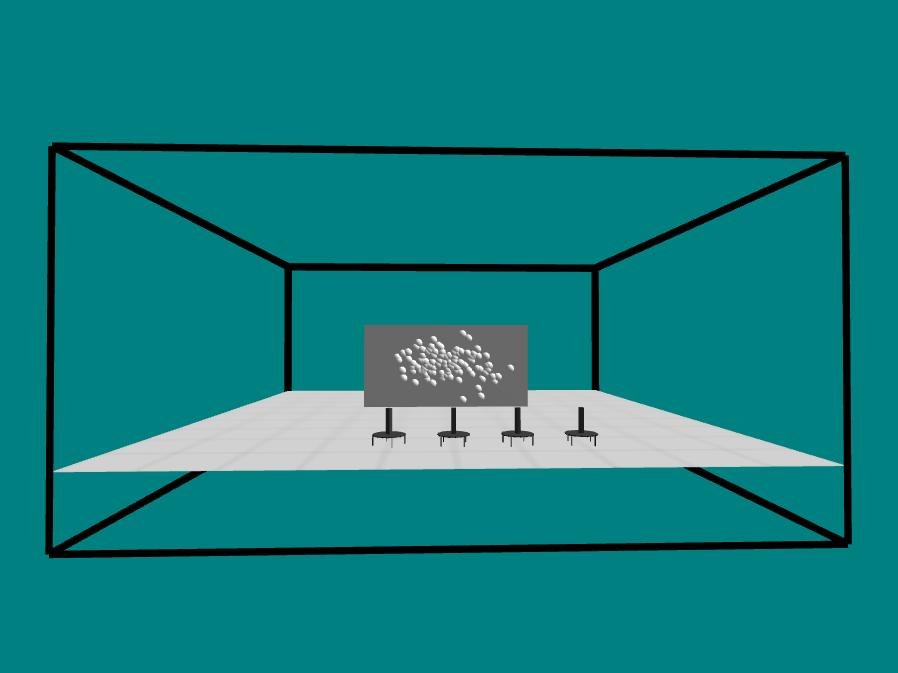
\includegraphics[width=\textwidth]{images/VerticalWallGardeningScene}
		\caption{Simulated Vertical Wall-Gardening Scene}
		\label{fig:sim_orig_scene}
		{The simulated vertical wall-gardening scene implemented and run in both control and experiment 	conditions. The vertical wall is laden with circular targets, functionally symbolic of leafed plants while the quadcopters are quadcopter-type eye-bots}.
	\end{subfigure}
	~
	\begin{subfigure}[b]{0.4\textwidth}
		\centering
		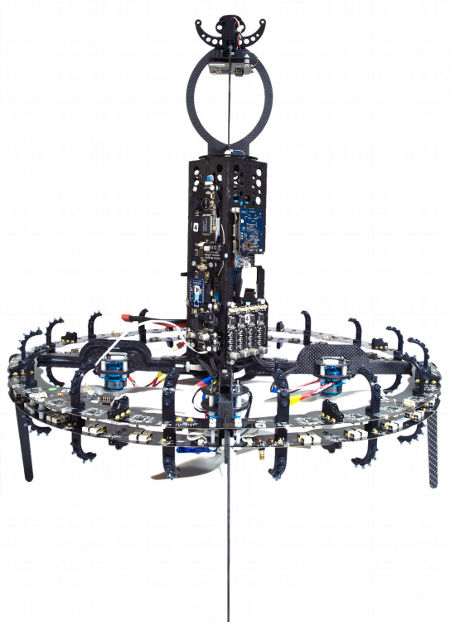
\includegraphics[width=\textwidth]{images/EyebotCarbonFrame}
		\caption{Eyebot Quadcopter}
		\label{fig:eyebot_hardware}
		{Image of a real-world Eyebot, designed and developed as a robotic agent in the Swarminoid Project \cite{Dorigo2013}}.
	\end{subfigure}
	\caption{Simulator Entities}
	\label{fig:sim_orig}
\end{figure}

The swarminoids' \cite{Dorigo2013} eye-bot quadcopter was selected as this studys' simulated, aerial platform due to its' established usage in heterogeneous swarm robotics research. By design, they are autonomous flying robots which can attach to an indoor ceiling, and are capable of analysing the environment from a privileged position to collectively gather information inaccessible to terrestrial-based robots \cite{Dorigo2013}. It is shown in \ref{fig:eyebot_hardware} and features the following sensing capabilities:
\begin{itemize}
    \item Custom 360° pan-tilt camera system, equipped with a 3MP camera.
    \item Optical 360° infrared environment distance scanner.
    \item Advanced 3D relative positioning sensor for swarm coordination/communication.
    \item Custom 6-Degree of freedom inertial sensing.
    \item Sonar and differential pressure sensors for altitude determination.
    \item Magnetometer for heading determination.
    \item Horizontal RGB led rings (local visual communication).
\end{itemize}

Additionally, both the control and experimental conditions employ a leader-based multi-agent strategy. PC Capabilities and threading?

\subsection{Uncertainties}
Assuring robot simulation realism is a growing focus area in graphical processing research with notable examples being AirSim \cite{Shah} and Morse \cite{Morse2011}.

\subsubsection{Robot and Target Positioning}
Kalman Filtering.
\subsubsection{Target Classification}
\subsubsection{Task and Target Uncertainties}

\subsection{Cooperative Control}

\subsubsection{Task Allocation}
Swarm robotics systems are characterised by decentralised control, limited communication between robots, use of local information and emergence of global behaviour \cite{Dorigo2013}.To design the organisation systems necessary for robot operation, the task space was delimited to 4 distinct domains:
\begin{itemize}
	\item Evaluation Task.
	\item Water Task.
	\item Nourish Task.
	\item Treatment Task.
\end{itemize}

\subsubsection{Behavioural Design}

\subsection{Path Planning}
Planning Parameters were kept constant for all experiments.

\bgroup
\def\arraystretch{1.5}% 
\begin{table}[h]
  \centering
  \begin{tabular}{|l|c|c|}
  \hline
  \textbf{Planner} & \textbf{Parameter Name} & \textbf{Parameter Value} \\
  \hline
  \multirow{3}{*}{PSO} & Self Trust & 0.2 \\
	& Past Trust & 0.1 \\
	& Global Trust & 0.7 \\
  \hline
  ACO & Number of Ants & 10 \\
  \hline
  \multirow{3}{*}{LAWN} & Launch Step & 500 \\
	& Horizontal Step & 0.1 \\
	& Vertical Step & 0.1 \\
  \hline
  \end{tabular}
  \caption{This table shows some data}
  \label{tab:myfirsttable}
\end{table}
\egroup

\subsubsection{Particle Swarm Optimization}
\subsubsection{Ant Colony Optimization}
\subsubsection{Lawn Sweeping Strategy}
Cao et al \cite{Cao1988} introduced a region filling strategy for sweeping operations in a robot lawn mower (RLM), thereby setting the stage for advanced studies into coverage path planning (CPP) strategies \cite{Galceran2013}. In this work, we implement the a similar region filling strategy, with one caveat being the lack of obstacle avoidance and replanning.

\section{Data Collection}

\chapter{Evaluation} \label{evaluation}

\chapter{Conclusion} \label{conclusion}
Future work into leaderless, self-organisation strategies with greater swarm sizes. The former can be achieved via agent roaming procedures that incorporate random walk behaviour with swarm cohesion implemented through Leinard-Jones potentials between agents.
Contributions include a programmatic framework for the generation of simulation data suitable for biological statistical analysis. A sample evaluation dataset is also made freely available for further inspection and analysis. Established path planners such as Open Motion Planning Library (OMPL) \cite{Sucan2012} should be considered for enhanced validity in comperative analyses. Further, higher order models of the quadcopter and external disturbances such as wind should be considered to enhance simulator realism. Higher order models are possible employing techniques to generating models learned from flight data \cite{Symington2014} whereas robust wind models such as the Dryden wind turbulence model \cite{Dryden} could be included. Collision detection and obstacle avaoidance with 3D-capable metaheuristic planners. Techniques and approaches to parameter optimisation and social learning such as genetic programming or neural networks are high potential, interest areas that would be considered to augment this work in future.
A standardised metaheuristic optimization algorithm library and a wider variety state prediction techniques such as probabilistic smoothing.
SLAM Mapping of targets.
Multi-objective TSP.
Enhanced local communication with the ring leds.
Implement time estimation techniques to vary holding times.
A dataset repository of similarly generated simulation data.

\appendix
\bibliographystyle{plain}
\bibliography{references/Library,references/Misc}
\chapter{Code listing}

\end{document}